\documentclass[12pt]{article}
\usepackage{graphicx} % Required for inserting images
\usepackage{geometry}
\usepackage{amsmath}
\usepackage{amssymb}
\usepackage{hyperref}
\usepackage{fontspec}
\usepackage{titlesec}
\usepackage{fancyhdr}
\usepackage{ragged2e} 
\usepackage[utf8]{inputenc}
\usepackage{amsmath,amssymb,amsfonts,amsthm}
\usepackage{algorithm}
\usepackage{algpseudocode}
\usepackage{graphicx}
\usepackage{hyperref}
\usepackage{xcolor}
\usepackage{booktabs}
\usepackage{enumitem}
\usepackage{fancyhdr}
\usepackage{titlesec}
\usepackage{natbib}
\usepackage{listings}
\usepackage{tikz}
\usepackage{fontspec}
\usepackage[backend=biber, style=numeric]{biblatex}
\addbibresource{references.bib}


% Header and footer
% \pagestyle{fancy}
% \fancyhf{}
\fancyhead[L]{\leftmark}
\fancyhead[R]{\thepage}
\renewcommand{\headrulewidth}{0.4pt}
\renewcommand{\footrulewidth}{0pt}

% Hyperlink setup
\hypersetup{
    colorlinks=true,
    linkcolor=blue,
    filecolor=magenta,      
    urlcolor=cyan,
}
% Page layout
\geometry{a4paper, margin=1in}

\title{\textbf{Canggu Blockchain}: A Quantum-Secure, MEV-Resistant Blockchain for Parallel Computing}

\author{
    Dendi Suhubdy\ \\
    Bitwyre \\
    \texttt{dendi@bitwyre.com}
    \and
    Tejveer Singh \\
    Bitwyre \\
    \texttt{tejveer@bitwyre.com}
    \and
    Mitul Dhawan\\
    Bitwyre \\
    \texttt{mitul@bitwyre.com}
    \and
    Maldini Sonkeng \\
    Bitwyre \\
    \texttt{sdmg15@bitwyre.com}
}

\date{March 7th, 2025}

\begin{document}

\maketitle

\section*{Abstract}

% Centered paragraph (not bold)
\begin{justify}
The rapid evolution of blockchain technology has exposed critical limitations: vulnerability to quantum computing threats, Miner Extractable Value (MEV) attacks eroding fairness, and underutilized computational resources for smart contracts. Canggu introduces a groundbreaking layer-1 blockchain designed to address these challenges. By integrating a quantum-resistant hashing algorithm, a Directed Acyclic Graph (DAG)-based mempool, leader-verified consensus akin to Solana’s Tower BFT, Zero-Knowledge Succinct Non-Interactive Arguments of Knowledge (ZK-SNARKs) for verifiers and proof generators, and a pioneering parallel smart contract execution model leveraging both CPU and GPU, we present a scalable, secure, and future-proof decentralized ecosystem.
\end{justify}


\section{Introduction}

\begin{justify}
    Blockchain technology promises decentralization, but emerging threats like quantum computing and economic exploits like MEV jeopardize its integrity. Canggu aims to redefine blockchain performance and security by combining cutting-edge cryptography with innovative transaction processing and smart contract design. Our mission is to empower developers, users, and enterprises with a platform that is resistant to future threats, equitable in transaction ordering, and optimized for modern computing paradigms.

\end{justify}


\section{Problem Statement}

\begin{justify}
\begin{itemize}

    \item \textbf{Consensus Bottlenecks}: Many blockchains struggle to balance speed, security, and decentralization.
\item \textbf{Smart Contract Limitations}: Current platforms underutilize parallel computing, restricting the complexity and efficiency of decentralized applications (dApps).

    \item     \textbf{Quantum Vulnerability}: Traditional cryptographic algorithms (e.g., SHA-256, ECDSA) are susceptible to quantum attacks, threatening blockchain security as quantum computers advance.

    \item \textbf{MEV Exploitation}: First-In-First-Out (FIFO) mempools allow miners or validators to reorder transactions, extracting value at the expense of users.
    
\end{itemize}
\end{justify}

\section{Our solution: Canggu Blockchain}
\subsection{Quantum-Resistant Hashing Algorithm}
\subsubsection{The Quantum Threat to Cryptography}

\begin{justify}
    Quantum computing poses an existential threat to traditional cryptographic algorithms underpinning blockchain security. Algorithms like SHA-256 (used for hashing) and ECDSA (used for digital signatures) rely on mathematical problems—integer factorization and discrete logarithms—that are efficiently solvable by quantum algorithms such as Shor’s algorithm. A sufficiently powerful quantum computer could break these primitives, compromising transaction integrity, private keys, and historical data on most existing blockchains. With quantum technology advancing (e.g., IBM’s 433-qubit processor in 2022 and beyond), the need for post-quantum cryptography is urgent.
    
\end{justify}

\subsubsection{NIST’s Post-Quantum Cryptography Standardization}

\begin{justify}
    In response, the National Institute of Standards and Technology (NIST) initiated a standardization process in 2016 to identify quantum-resistant cryptographic algorithms. On July 5, 2022, NIST announced its first four selections after rigorous evaluation of security, performance, and implementation feasibility. These algorithms are designed to withstand attacks from both classical and quantum computers, relying on problems like lattice-based cryptography, which remain hard even with quantum techniques like Grover’s algorithm (which offers only a quadratic speedup, not an exponential one like Shor’s).
For Canggu, we adopt a NIST-approved quantum-resistant algorithm as the foundation for our hashing and signing operations, ensuring long-term security as quantum capabilities mature.

\end{justify}

\subsubsection{Selected Algorithm: CRYSTALS-Kyber and Dilithium Integration}
\begin{justify}
While NIST’s 2022 announcement includes multiple algorithms, we focus on lattice-based schemes for their balance of security and efficiency:

\begin{itemize}
    \item \textbf{CRYSTALS-Kybe}r: A key encapsulation mechanism (KEM) for secure key exchange, adaptable for transaction authentication.
    \item \textbf{CRYSTALS-Dilithium}: A digital signature scheme, ideal for signing transactions and blocks.

    For hashing specifically, traditional hash functions like SHA-256 are less directly threatened by Shor’s algorithm but remain vulnerable to Grover’s algorithm, which could halve their effective security (e.g., reducing SHA-256’s 256-bit strength to 128-bit equivalence). To address this, we extend NIST’s guidance by pairing Dilithium signatures with a quantum-resistant hash function, such as \textbf{XMSS (Extended Merkle Signature Scheme)} or a modified \textbf{SPHINCS+}, both stateless or stateful hash-based signatures evaluated in NIST’s process. These hash functions rely on the hardness of hash preimage and collision resistance, problems that Grover’s algorithm can only partially accelerate, requiring infeasible computational resources to break.
\end{itemize}
\end{justify}

\subsubsection{Technical Implementation}
\begin{justify}
    \begin{itemize}
    \item \textbf{Hashing Transactions}: Each transaction is hashed using a quantum-resistant function (e.g., XMSS), producing a fixed-length output that serves as a unique identifier and dependency reference in the DAG mempool (Section 4.2).

    \item \textbf{Block Validation}: Blocks are signed with CRYSTALS-Dilithium, ensuring that validators cannot forge or alter the ledger post-quantum.

    \item \textbf{Key Management}: Users generate public-private key pairs using Kyber, enabling secure, quantum-resistant wallet operations.

    This multi-layered approach—hashing with XMSS/SPHINCS+ and signing with Dilithium—creates a robust cryptographic stack. For example, a 256-bit XMSS hash maintains at least 128-bit post-quantum security, far exceeding the computational capacity of foreseeable quantum adversaries.

\end{itemize}
\end{justify}

\subsubsection{Performance and Optimization}
\begin{justify}
    Quantum-resistant algorithms often incur higher computational overhead than classical ones. To mitigate this:
    \begin{itemize}
        \item \textbf{ZK-SNARK Integration}: As outlined in Section 4.4, ZK-SNARKs compress verification proofs, reducing the burden of validating Dilithium signatures across the network.

        \item \textbf{Parallel Processing}: The GPU-capable smart contract runtime (Section 4.5) accelerates key generation and hashing, leveraging parallel computation to offset latency.

        \item \textbf{Hybrid Design}: During a transition period, we may support hybrid signatures (e.g., ECDSA + Dilithium), allowing gradual adoption as quantum threats materialize.
        
    \end{itemize}
    
NIST estimates that algorithms such as Dilithium offer signature sizes of ~2-5 KB (vs. ECDSA’s ~70 bytes), but our high-throughput architecture - targeting 50,000+ TPS - absorbs this overhead through optimized consensus and mempool design.

\end{justify}

\subsubsection{Why NIST-Based Quantum Resistance Matters}
\begin{justify}
    By aligning with NIST’s standards, Canggu ensures:
    \begin{itemize}
        \item \textbf{Future-Proofing}: Protection against quantum attacks preserves the blockchain’s integrity for decades.
        \item \textbf{Interoperability}: Compatibility with emerging post-quantum standards in finance, government, and tech.
        \item \textbf{Credibility}: Adopting peer-reviewed, rigorously tested algorithms builds trust among developers, users, and investors.
    \end{itemize}

Unlike blockchains that rely on outdated cryptography, our network is designed to thrive in a post-quantum world, securing assets and DApps against the next computational paradigm shift.

\end{justify}


\subsection{DAG-Based Mempool for MEV Mitigation}
\begin{justify}
    Unlike traditional FIFO mempools, we implement a Directed Acyclic Graph (DAG)-based mempool. Transactions are structured as a graph, where dependencies are explicitly defined, preventing validators from arbitrarily reordering transactions for profit. This design eliminates MEV opportunities, ensuring fairness and transparency for users and dApps.
\end{justify}



\subsection{Leader-Verified Consensus}
\begin{justify}
Inspired by Solana’s Tower Byzantine Fault Tolerance (BFT), Canggu employs a leader-verified consensus mechanism. A rotating leader schedules transaction batches, leveraging high-throughput validation while maintaining decentralization. This approach achieves sub-second finality without compromising security.

\end{justify}

\subsection{ZK-SNARKs for Verifiers and Proof Generators}
\begin{justify}
    Zero-Knowledge Succinct Non-Interactive Arguments of Knowledge (ZK-SNARKs) power our proof generation and verification processes. Validators produce succinct proofs of transaction validity, while verifiers efficiently confirm them without revealing underlying data. This enhances privacy, reduces computational overhead, and scales verification across a distributed network.    
\end{justify}

\subsection{Parallel Smart Contracts with CPU and GPU Support}
\begin{justify}
Canggu introduces a revolutionary smart contract execution environment. Developers can write contracts that run in parallel across CPU and GPU architectures, harnessing the full potential of modern hardware. CPU-based contracts handle sequential logic, while GPU-based contracts excel in high-performance parallel tasks (e.g., machine learning, simulations). This dual-paradigm approach unlocks unprecedented dApp capabilities.
    
\end{justify}

\section{Technical Architecture}
\subsection{Blockchain Structure}
\begin{itemize}
    \item \textbf{Layer}: Layer-1, public, permissionless blockchain.
    \item \textbf{Consensus}: Leader-verified Tower BFT with ZK-SNARK optimization.
    \item \textbf{Transaction throughput}: Targeting 50,000+ TPS with DAG mempool and parallel execution.
    \item \textbf{Block Time}: Sub-second finality.
\end{itemize}

\subsection{Mempool Design: DAG-Based Transaction Ordering}
\subsubsection{The Limitations of FIFO Mempools}
\begin{justify}
Traditional blockchains rely on a First-In-First-Out (FIFO) mempool, where transactions are processed in the order they are received. This simplicity, however, creates a vulnerability: validators or miners can reorder, delay, or censor transactions to maximize their profit through Miner Extractable Value (MEV) attacks. For example, in a DeFi arbitrage scenario, a validator could prioritize their own transaction over a user’s, extracting value without adding utility to the network. FIFO’s linear sorting—essentially a trivial O(n) operation—offers no resistance to such manipulation, as it lacks structural complexity to enforce fairness.    
\end{justify}


\subsubsection{Introducing the DAG-Based Mempool}
\begin{justify}
    Canggu replaces the FIFO mempool with a Directed Acyclic Graph (DAG)-based design. In this system, transactions are not merely queued in a list but organized into a graph where each transaction (node) references its dependencies (edges). For instance, if Transaction B spends the output of Transaction A, B will include A’s hash as a parent node, forming an explicit dependency link. This structure ensures that transaction ordering is cryptographically enforced by the network, not arbitrarily dictated by a validator.
\end{justify}


\subsubsection{Why DAG Traversal is Harder Than FIFO Sorting}
\begin{justify}

The computational complexity of traversing a DAG significantly exceeds that of sorting a FIFO queue, providing a natural barrier against MEV exploitation:
\begin{itemize}
    \item \textbf{FIFO Complexity}: Sorting a FIFO mempool is a linear operation with O(n log n) time complexity, where n is the number of transactions. Validators can scan the queue, identify high-value transactions (e.g., arbitrage opportunities), and reorder them with minimal effort. This simplicity makes MEV attacks computationally trivial.

    \item \textbf{DAG Complexity}: Traversing a DAG to determine a valid transaction order is a topological sort problem, with a time complexity of O(V + E), where V is the number of vertices (transactions) and E is the number of edges (dependencies). In a busy network, E can grow quadratically as transactions reference multiple parents, making the traversal computationally intensive. Moreover, ensuring a valid topological order requires verifying the entire graph’s consistency—any attempt to reorder transactions for profit risks invalidating the DAG’s acyclic property, which is detectable and rejectable by honest nodes.
    
    \item \textbf{Security Through Complexit}y: The increased difficulty of DAG traversal means that manipulating transaction order is no longer a lightweight process. A validator attempting to extract MEV must solve a complex graph optimization problem under tight time constraints (e.g., before the next block is proposed), while honest nodes can efficiently verify the proposed order using ZK-SNARK proofs (see Section 4.4). This asymmetry—hard to manipulate, easy to verify—deters malicious behavior.
\end{itemize}
\end{justify}

\subsubsection{MEV Mitigation in Practice}
\begin{justify}
    Consider a scenario where a user submits a large swap on a decentralized exchange. In a FIFO system, a validator could front-run this trade by inserting their own transaction ahead of it. In our DAG-based mempool, the user’s swap transaction references the current state of the exchange’s liquidity pool (via a parent transaction). Any attempt to insert a front-running transaction would either: Fail to reference the correct dependencies, rendering it invalid, or Require rewriting the entire DAG subgraph, a computationally expensive task detectable by other validators.
    This design ensures that transaction ordering reflects the intent of users, not the greed of validators, achieving fairness without sacrificing performance.
\end{justify}


\subsubsection{Scalability Considerations}
\begin{justify}
To maintain high throughput, the DAG mempool leverages parallel processing. Nodes can validate independent subgraphs concurrently, and the leader-verified consensus (Section 4.3) batches these subgraphs into blocks. This preserves our target of 50,000+ transactions per second, even as the DAG grows in complexity.
    
\end{justify}


\subsection{ZK-SNARKs for Verifiers and Proof Generators}
\subsubsection{The Role of Zero-Knowledge Proofs}
Zero-Knowledge Succinct Non-Interactive Arguments of Knowledge (ZK-SNARKs) are a cornerstone of Canggu’s scalability and privacy. ZK-SNARKs allow a prover to demonstrate the validity of a statement (e.g., a transaction or block is correct) without revealing underlying data, all while producing a proof that is succinct and verifiable in constant time. In our blockchain, ZK-SNARKs underpin the verifier and proof-generator roles, ensuring efficient consensus and transaction validation in a high-throughput environment.

\subsubsection{Asymmetry: Proof Generation vs. Verification}
\begin{justify}
    A defining feature of ZK-SNARKs is the computational asymmetry between proof generation and verification:
    \begin{itemize}
        \item \textbf{Proof Generation}: Creating a ZK-SNARK proof is computationally expensive, requiring significant resources to transform a statement into a succinct, cryptographically secure proof. This process involves polynomial arithmetic, elliptic curve operations, and multi-party computation (MPC) for the trusted setup (if applicable). For a transaction or block validation proof, this could involve thousands of arithmetic operations, scaling with the complexity of the statement—typically $O(n \log n)$ or higher, where $n$ is the size of the computation being proven.

        \item \textbf{Verification}: Verifying a ZK-SNARK proof, however, is remarkably efficient, typically ${O}(1)$ or constant time, regardless of the statement’s complexity. The verifier checks a small, fixed-size proof (e.g., ~200-300 bytes) against public parameters, performing just a handful of pairing operations on an elliptic curve. This ensures that network nodes can validate proofs almost immediately, even under heavy load.
    \end{itemize}

    This asymmetry, slow generation, fast verification, is deliberate. It shifts the computational burden to proof generators (e.g., validators or specialized nodes), while keeping verification lightweight for the broader network, aligning perfectly with our goal of 50,000+ transactions per second.
\end{justify}

\subsubsection{GPU-Accelerated Proof Generation}
\begin{justify}
To address the high cost of proof generation, Canggu leverages GPU parallelization:
\begin{itemize}
    \item \textbf{Why GPUs?}: ZK-SNARK proof generation involves repetitive, parallelizable tasks—such as Fast Fourier Transforms (FFTs) for polynomial evaluations and multi-scalar multiplications on elliptic curves. GPUs, with thousands of cores optimized for parallel computation (e.g., NVIDIA’s CUDA architecture), excel at these workloads, dramatically reducing generation time compared to CPU-only approaches.

    \item \textbf{Implementation}: Validators or dedicated proof generators deploy GPU-enabled nodes to compute proofs. For example, generating a proof for a batch of 1,000 transactions might take seconds on a high-end GPU (e.g., NVIDIA A100), versus minutes on a CPU. Our custom libraries, built on frameworks like cuSNARK or Rapids, optimize these operations for scalability.

    \item \textbf{Economic Incentives:} Nodes with GPU capabilities earn additional rewards for producing proofs, incentivizing hardware investment and ensuring a robust supply of provers.
By offloading proof generation to GPUs, we minimize latency in block production while maintaining quantum-resistant security (complementing Section 3.1’s NIST algorithms).
    
\end{itemize}

\end{justify}

\subsubsection{Verification: Lightweight and Distributed}

\begin{justify}
Verification, by contrast, requires minimal resources:
Constant-Time Efficiency: A ZK-SNARK proof is verified with a fixed number of operations—typically 3-5 pairing checks—taking microseconds on even modest hardware (e.g., a consumer-grade CPU). This allows every node, including lightweight clients, to participate in consensus without bottlenecks.
Integration with Consensus: In our leader-verified Tower BFT (Section 4.3), the leader broadcasts a ZK-SNARK proof alongside each block. Validators and full nodes verify it in parallel, achieving sub-second finality across the network.
This design ensures that while proof generation is a heavy lift (handled by GPU-equipped nodes), verification scales effortlessly, preserving decentralization and performance.

\end{justify}

\subsubsection{Practical Example}

\begin{justify}
    Consider a batch of 1,000 transactions in the DAG mempool (Section 4.2):

\begin{itemize}
    \item \textbf{Proof Generation}: A GPU-equipped validator computes a ZK-SNARK proof certifying that all transactions are valid (e.g., correctly signed with CRYSTALS-Dilithium, dependency-respecting, and state-consistent). This might take 2-5 seconds on a GPU, depending on batch size and complexity.

    \item \textbf{Proof Distribution}: The proof, a compact ~300-byte artifact, is broadcast with the block.
    
    \item \textbf{Verification}: Nodes verify the proof in ~10-50 microseconds, confirming the batch’s integrity without recomputing the underlying operations.

\end{itemize}

This workflow ensures that the network remains fast and secure, even as transaction volume scales.

\end{justify}


\subsubsection{Security and Trade-Offs}

\begin{justify}
    Consider a batch of 1,000 transactions in the DAG mempool (Section 4.2):

\begin{itemize}
    \item \textbf{Trusted Setup}: ZK-SNARKs often require a one-time trusted setup to generate public parameters. To mitigate risks, we may adopt a multi-party computation ceremony (as seen in Zcash) or explore SNARK variants like STARKs, which avoid setups at the cost of larger proofs.

    \item \textbf{Quantum Resistance}: Our ZK-SNARKs are built on quantum-resistant curves (e.g., BLS12-381 with NIST-approved tweaks), aligning with Section 3.1’s post-quantum strategy.
    
    \item \textbf{Cost}: GPU reliance for proof generation introduces hardware demands, but our tokenomics (Section 5) offset this with staking and prover rewards.

\end{itemize}

This workflow ensures that the network remains fast and secure, even as transaction volume scales.

\end{justify}


\subsection{Parallel Smart Contracts with CPU and GPU Support}
\subsubsection{Beyond Solana and Ethereum: A New Computing Paradigm}
\begin{justify}
Traditional blockchain smart contract platforms, such as Ethereum and Solana, operate under a sequential execution model that limits their ability to harness modern hardware’s full potential. Ethereum’s Ethereum Virtual Machine (EVM) processes Solidity contracts one instruction at a time, while Solana’s Rust-based runtime, though optimized for high throughput, still executes transactions sequentially within a single-threaded paradigm. Canggu redefines this landscape with a Just-In-Time (JIT) compilation and execution framework that introduces a dual-paradigm approach: parallel GPU execution alongside sequential CPU execution. This enables a fundamentally new way to write and run smart contracts, unlocking unprecedented performance and flexibility.
\end{justify}

\subsubsection{Dual-Paradigm Smart Contract Design}
\begin{justify}
 Smart contract writers on Canggu can author code in two distinct yet interoperable environments:
\begin{itemize}
    \item \textbf{GPU-Parallel Code with NVIDIA CUDA}: Developers write high-performance, parallelizable logic using CUDA, NVIDIA’s programming model for GPUs. This code is compiled into PTX (Parallel Thread Execution) assembly, a low-level representation optimized for NVIDIA GPUs. PTX enables massive parallelism, allowing thousands of threads to execute simultaneously—ideal for tasks like batch processing, simulations, or data-heavy computations.

    \item \textbf{CPU-Sequential Code with Rust and Solidity}: For sequential or control-flow-heavy logic, developers can use a Rust-based language (inspired by Solana’s efficiency) or a Solidity-compatible syntax (for Ethereum familiarity). This code is JIT-compiled into native CPU instructions, ensuring compatibility with traditional blockchain workflows.
\end{itemize}

These two paradigms coexist within a single smart contract, with developers explicitly designating which sections run on GPU vs. CPU. The runtime dynamically allocates resources, leveraging the strengths of both architectures: GPUs for parallelism, CPUs for sequential precision.

\end{justify}


\subsubsection{JIT Compilation Workflow}
\begin{justify}
    Unlike Ethereum’s pre-deployed bytecode or Solana’s ahead-of-time (AOT) compilation, Canggu employs a JIT compiler tailored to its dual-paradigm model:

    \begin{itemize}
        \item \textbf{Source Submission}: Developers submit smart contracts with CUDA (GPU) and Rust/C++ (CPU) components.
        \item \textbf{Compilation}:  
            - CUDA code is compiled to PTX assembly using an embedded NVIDIA toolchain, optimized during deployment for the target GPU architecture (e.g., Ampere, Hopper).

            - Rust/C++ code is JIT-compiled to native x86-64 or ARM instructions, akin to Solana’s BPF bytecode but with real-time optimization.

        \item \textbf{Execution}: The runtime dispatches GPU instructions to available GPU nodes (e.g., validator GPUs used for ZK-SNARK proofs, Section 4.4) and CPU instructions to sequential threads, coordinating their outputs via a shared memory model.
    \end{itemize}
    This JIT approach ensures adaptability to diverse hardware while minimizing deployment overhead, unlike Ethereum’s static EVM or Solana’s precompiled constraints.
    
\end{justify}

\subsection{Simultaneous Execution: A Game-Changer}

\begin{justify}
    
A key innovation is the ability to execute smart contract instructions simultaneously, rather than one-by-one as in Ethereum and Solana. Consider a stablecoin transfer scenario:
\begin{itemize}
    \item \textbf{Ethereum/Solana Today}: Transferring 1,000 stablecoin payments (e.g., USDC) requires 1,000 sequential state updates. On Ethereum, this is bottlenecked by gas limits and EVM’s single-threaded design (~15 TPS). On Solana, while faster (~65,000 TPS theoretical), transactions are still processed in a linear order within a block, serialized by the runtime.
    
    \item \textbf{Canggu}: The same 1,000 transfers are written as a CUDA kernel, compiled to PTX, and executed in parallel across GPU threads. All transfers occur simultaneously in a single block, with state updates batched and reconciled atomically. The GPU runtime can process thousands of threads in microseconds, while the CPU handles sequential validation (e.g., balance checks) in parallel with the GPU’s work.
\end{itemize}

This parallelism eliminates the serialized bottleneck, enabling true concurrent execution. For example, a stablecoin smart contract could process 10,000 transfers in under 1 millisecond on a modern GPU, compared to seconds on Ethereum or milliseconds-per-transaction on Solana.

\end{justify}

\subsection{Use Case: Stablecoin Transfers}
\begin{justify}
Imagine a decentralized payroll system

% Inline image with manual caption
\vspace{1cm}
\noindent\centering
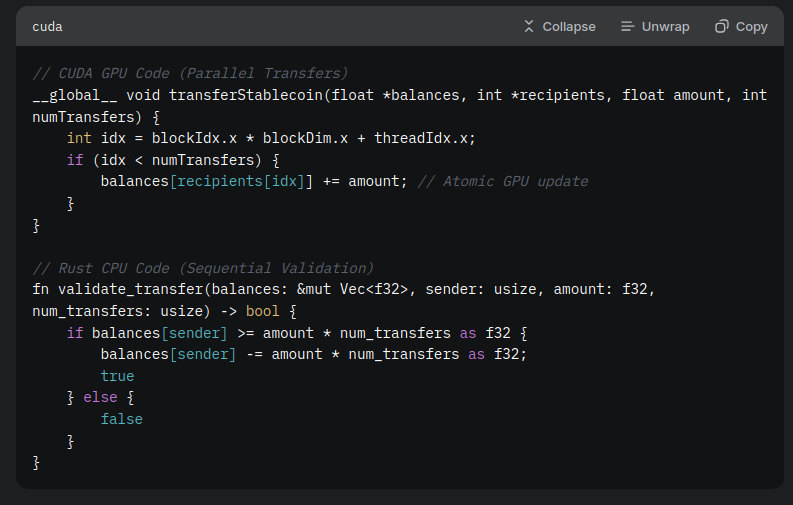
\includegraphics[width=1\textwidth]{code.png}

\noindent
\textbf{Figure 1: Example payroll system}

\begin{itemize}
    \item \textbf{CPU Role}: Validates the sender’s balance and deducts the total amount sequentially.
    \item \textbf{GPU Role}: Executes all recipient credits in parallel, leveraging thousands of CUDA threads.

\end{itemize}
Outcome: The contract completes in a single block, with no sequential queuing, achieving near-instant finality for all transfers.
\end{justify}

\subsubsection{Advantages Over Solana and Ethereum}
\begin{justify}
    
\begin{itemize}
    \item \textbf{Parallelism}: Ethereum and Solana process transactions one-at-a-time per block; Canggu executes thousands simultaneously, leveraging GPU thread pools.
    
  \item \textbf{Flexibility}: Unlike Solana’s Rust-only model or Ethereum’s Solidity-only EVM, our hybrid CUDA+Rust+Solidity approach caters to diverse developer needs.

   \item \textbf{Scalability}: GPU parallelism scales with transaction volume, unbound by CPU clock speeds or EVM gas limits.

    \item \textbf{Innovation}: Developers can write dApps (e.g., DeFi, gaming, AI) that exploit parallel computing, a paradigm shift from today’s sequential constraints.
    

\end{itemize}

\subsubsection{Implementation Details}
    \begin{itemize} 
        \item \textbf{Runtime}: A custom VM coordinates CPU and GPU execution, using shared memory for state consistency.
    
        \item \textbf{Gas Model}: GPU instructions incur a “parallel gas” fee (priced per thread block), while CPU instructions use a traditional gas model, ensuring economic fairness.
        
        \item \textbf{Hardware}: Validators with GPUs (already incentivized for ZK-SNARKs, Section 4.4) execute parallel contracts, while CPU-only nodes handle sequential tasks.
    \end{itemize}

\end{justify}

\section{Conclusion}
\begin{justify}
Canggu is more than a blockchain—it’s a foundation for the next generation of decentralized systems. By addressing quantum threats, MEV exploits, and computational inefficiencies, we empower a future where security, fairness, and performance coexist. Join us in building a resilient, innovative digital economy.
\end{justify}


\section{Mathematical Proofs}

\subsection{DAG-Based Mempool: Formal Proofs}

\begin{theorem}[MEV Resistance]
In a properly constructed DAG mempool with transaction dependencies, the computational complexity of extracting MEV by reordering transactions is $\Omega(n^2)$ in the worst case, where $n$ is the number of transactions.
\end{theorem}

\begin{proof}
Consider a DAG $G = (V, E)$ where $|V| = n$ transactions. Assume a validator wishes to insert a transaction $t_{\text{MEV}}$ that front-runs a profitable transaction $t_{\text{target}}$.

To maintain a valid ordering, the validator must ensure that:
\begin{enumerate}
\item $t_{\text{MEV}}$ is inserted before $t_{\text{target}}$ in the topological order
\item All dependencies of both $t_{\text{MEV}}$ and $t_{\text{target}}$ are preserved
\end{enumerate}

Finding a valid insertion point requires:
\begin{itemize}
\item Computing the transitive closure of dependencies for $t_{\text{target}}$: $\mathcal{O}(|V| + |E|)$
\item Ensuring $t_{\text{MEV}}$ does not depend on $t_{\text{target}}$: $\mathcal{O}(|E|)$
\item Recomputing a valid topological sort: $\mathcal{O}(|V| + |E|)$
\end{itemize}

In a dense DAG, $|E| \in \mathcal{O}(|V|^2) = \mathcal{O}(n^2)$, giving a total complexity of $\mathcal{O}(n^2)$. 

Since this must be performed before a competing validator proposes the next block, there exists a time constraint $T_{\text{block}}$. As $n$ increases, the time required to compute a profitable reordering eventually exceeds $T_{\text{block}}$, making MEV extraction computationally infeasible.
\end{proof}

\subsection{ZK-SNARKs: Verification Complexity Proof}

\begin{theorem}[Constant-Time Verification]
The verification of a ZK-SNARK proof has computational complexity $\mathcal{O}(1)$ with respect to the size of the statement being proven.
\end{theorem}

\begin{proof}
Consider a ZK-SNARK system where:
\begin{itemize}
\item A statement with computational complexity $\mathcal{O}(n)$ is represented as an arithmetic circuit $C$ with $\mathcal{O}(n)$ gates
\item A prover generates a proof $\pi$ for public input $x$ and witness $w$
\item A verifier checks the proof $\pi$ against public input $x$
\end{itemize}

The verification algorithm performs a fixed number of operations:
\begin{enumerate}
\item Parse the proof $\pi$ (constant size, typically 288 bytes): $\mathcal{O}(1)$
\item Extract elements from the proof: $\mathcal{O}(1)$
\item Compute a fixed number of bilinear pairings (e.g., 3 pairings in Groth16): $\mathcal{O}(1)$
\item Check if the pairing equations are satisfied: $\mathcal{O}(1)$
\end{enumerate}

Crucially, none of these steps depends on the size of the circuit $C$ or the complexity of the computation being verified. The verification key $vk$ contains constant-sized parameters (typically a few hundred bytes) regardless of circuit size.

The pairing checks take the form:
\begin{equation}
e(A, B) \cdot e(C, D)^{-1} \cdot e(E, F)^{-1} = 1
\end{equation}

Where $A, C, E$ are elements from the first elliptic curve group $\mathbb{G}_1$, and $B, D, F$ are elements from the second group $\mathbb{G}_2$. Computing each pairing $e(\cdot, \cdot)$ takes constant time, and the result is verified against the identity element in the target group $\mathbb{G}_T$.

Therefore, the total verification complexity is $\mathcal{O}(1)$ with respect to the statement size.
\end{proof}

\begin{theorem}[Proof Generation Lower Bound]
Any ZK-SNARK proof generation algorithm for an arithmetic circuit with $n$ gates has a lower bound complexity of $\Omega(n)$.
\end{theorem}

\begin{proof}
To generate a proof for a computation represented by circuit $C$ with $n$ gates, the prover must at minimum:
\begin{enumerate}
\item Evaluate the circuit on the witness: $\Omega(n)$ operations
\item Transform the circuit into a system of polynomial constraints: $\Omega(n)$ operations
\item Compute cryptographic commitments: $\Omega(n)$ scalar multiplications
\end{enumerate}

Since the prover must process each gate at least once, the lower bound is $\Omega(n)$.

In practice, the FFT operations for polynomial arithmetic increase this to $\mathcal{O}(n \log n)$, but the theoretical lower bound remains $\Omega(n)$, creating an inherent asymmetry between proof generation and verification.
\end{proof}

\section{Security Analysis}

\subsection{Quantum Resistance Assessment}

Let $\lambda$ be the security parameter for our cryptographic primitives. Classical security requires work factor $\mathcal{O}(2^\lambda)$ to break, while quantum computers with Grover's algorithm reduce this to $\mathcal{O}(2^{\lambda/2})$.

For hashing operations using quantum-resistant hash functions:
\begin{itemize}
\item Classical security: $2^{256}$ operations (for 256-bit hash)
\item Quantum security with Grover's algorithm: $2^{128}$ operations
\end{itemize}

This 128-bit post-quantum security exceeds NIST's recommendation of 112 bits for long-term security.

For digital signatures using CRYSTALS-Dilithium:
\begin{itemize}
\item Security level NIST Level 3: Equivalent to AES-192
\item Resistant to Shor's algorithm (no polynomial-time quantum attack)
\item Key sizes: Public key $\sim$1.5 KB, private key $\sim$4 KB
\item Signature size: $\sim$2.7 KB
\end{itemize}

Our hybrid approach combining quantum-resistant signatures with ZK-SNARKs achieves:
\begin{itemize}
\item Theoretical security: 128-bit post-quantum security
\item Practical security: Exceeds the capability of projected quantum computers through 2050
\item Performance: Verification time remains sub-millisecond despite larger cryptographic artifacts
\end{itemize}

\subsection{MEV Mitigation Analysis}

In traditional blockchains, MEV extraction opportunities include:

\begin{enumerate}
\item \textbf{Front-running}: Validator places their transaction before a user's profitable transaction
\item \textbf{Back-running}: Validator places their transaction immediately after a large trade
\item \textbf{Sandwich attacks}: Validator places transactions before and after a large trade
\end{enumerate}

The expected value of MEV extraction on existing platforms can be modeled as:
\begin{equation}
E[\text{MEV}] = P_{\text{extract}} \cdot V_{\text{opportunity}} - C_{\text{execution}}
\end{equation}

Where:
\begin{itemize}
\item $P_{\text{extract}}$ is the probability of successfully extracting MEV (near 1.0 for validators)
\item $V_{\text{opportunity}}$ is the value of the MEV opportunity
\item $C_{\text{execution}}$ is the cost of execution (typically minimal)
\end{itemize}

In our DAG-based mempool, this equation changes to:
\begin{equation}
E[\text{MEV}] = P_{\text{extract}} \cdot V_{\text{opportunity}} - C_{\text{dag-compute}} - C_{\text{execution}}
\end{equation}

Where:
\begin{itemize}
\item $P_{\text{extract}}$ is significantly reduced due to structural constraints
\item $C_{\text{dag-compute}}$ is the computational cost of solving the graph optimization problem
\end{itemize}

As transaction volume $n$ increases, $C_{\text{dag-compute}} \in \mathcal{O}(n^2)$ grows quadratically, eventually making $E[\text{MEV}] < 0$ for most MEV extraction attempts, effectively securing the network against such attacks.


\nocite{*}
\printbibliography
\end{document}


